\documentclass[12pt]{article}
\usepackage[utf8]{inputenc}
\usepackage[italian]{babel}
\usepackage[margin=0.5in]{geometry}
\usepackage{tocloft}
\usepackage{graphicx}
\usepackage{longtable}
\usepackage{pdflscape}
\usepackage{array}
\usepackage{float}
\usepackage{textcomp}
\usepackage{hyperref}

\usepackage{alltt}

\usepackage{lipsum} % da cancellare

\usepackage{multicol}
\usepackage{booktabs}

\cftsetindents{section}{0em}{2em}
\cftsetindents{subsection}{0em}{2em}

\renewcommand\cfttoctitlefont{\hfill\Huge}
\renewcommand\cftaftertoctitle{\hfill\mbox{}}
\renewcommand\arraystretch{1.5}

% Itemize senza separatore
\let\olditemize\itemize
\renewcommand\itemize{\olditemize\setlength{\itemsep}{0pt}}

% Itemize senza separatore, spazio sopra/sotto dimezzato
% \let\olditemize\itemize
% \let\oldenditemize\enditemize
% \renewcommand\itemize{\vspace{-.5\topsep}\olditemize\setlength{\itemsep}{0pt}}
% \renewcommand\enditemize{\oldenditemize\vspace{-.5\topsep}}

\def\labelitemi{--}

\begin{document}

%=================================================================
% 						TITLE PAGE
%=================================================================
\begin{titlepage}

\newcommand{\HRule}{\rule{\linewidth}{0.2mm}}

\center
\vspace*{1cm\vfill}
\textsc{\LARGE Università degli studi di Padova}\\[4.5cm] 
\textsc{\Large Progetto di Tecnologie Web}\\[1cm]


\HRule \\[0.4cm]
{ \huge Piattaforma TutorHub}\\[0.15cm] 
\HRule \\[1.5cm]
 

\begin{minipage}{0.4\textwidth}
\begin{flushleft} \large
	\textsc{Aaron Cesaro} \\
	\textsc{Mustafa Hafidi} 
\end{flushleft}
\end{minipage}
~
\begin{minipage}{0.4\textwidth}
\begin{flushright} \large
	\textsc{Andrea Biondo}  \\
	\textsc{Michele Antonazzi}
\end{flushright}
\end{minipage}\\[4cm]

\vspace{\fill}

{\large \today}
\end{titlepage}


%=================================================================
% 						TABLE OF CONTENTS
%=================================================================

\tableofcontents
\newpage



%=================================================================
% 						ABSTRACT PAGE
%=================================================================
\section*{Abstract}
\emph{TutorHub} \`e una piattaforma online creata alla scopo di facilitare la gestione dei rapporti tra insegnanti di ripetizioni ed alunni. Grazie a \emph{TutorHub} gli studenti potranno cercare l'insegnante pi\`u adatto alle loro esigenze, mentre i tutors disporranno di un comodo strumento per la gestione delle lezioni che danno, oltre alla possibilit\`a di rendere pubbliche le proprie conoscenze e tariffe, incrementando cos\`i il numero degli studenti interessati a ricevere ripetizioni.

%=================================================================
%	 						REQUISITI
%=================================================================
\section{Analisi dei requisiti}

\subsection{Categorie di utenti}
Le categorie di utenti a cui \`e rivolto il sito sono principalmente due:
\begin{itemize}
	\item utenti interessati a ricevere lezioni private (alunni);
	\item utenti interessati a erogare lezioni private (insegnanti).
\end{itemize}
Mentre la prima categoria di utenti si \`e ritenuto essere per lo pi\`u omogenea, la seconda risulta estremamente eterogenea. A questa seconda categoria infatti appartengono persone di entrambi i sessi con un'et\`a compresa tra i 20 ed i 60 anni. Tra questi sono presenti figure come:

\begin{itemize}
	\item studenti universitari;
	\item ricercatori;
	\item insegnanti;
	\item professionisti di settore.
\end{itemize}

\subsection{Obiettivi per classe di utenza}
A causa di questa eterogeneit\`a \`e stato necessario rendere la piattaforma il pi\`u semplice ed intuitiva possibile. Si \`e infatti tenuto conto sia delle difficolt\`a degli utenti pi\`u anziani, che generalmente hanno pi\`u difficolt\`a nell'utilizzo del web, che degli utenti con disabilit\`a. La progettazione ha quindi preso la direzione della semplicit\`a, cercando in primis di privilegiare la chiarezza e l'intuitivit\`a delle funzionalit\`a.

\subsubsection{Utente Tutor}
A questa prima tipologia corrispondono gli utenti che vorrebbero rendersi disponibili per fornire delle lezioni a pagamento ad altri utenti della piattaforma.
Per ogni tutor \`e necessario memorizzare e gestire le seguenti informazioni:
\begin{itemize}
	\item  disponibilità:
		\begin{itemize}
			\item Fascia oraria;
			\item Giorni;
		\end{itemize}
	\item materie: l'insieme delle materie che l'utente è disposto ad insegnare comprensive del prezzo.
\end{itemize}

\subsubsection{Materie}
Ogni tutor pu\`o aggiungere le materie che desidera insegnare. In particolare ogni materia deve avere le seguenti informazioni:
\begin{itemize}
	\item nome;
	\item prezzo orario.
\end{itemize}
Le materie inserite dai tutor vengono salvate in modo persistente sul database per poi essere riproposte sotto forma di suggerimenti al momento della ricerca da parte degli alunni o durante l'inserimento della materia da parte dei tutor.

\subsubsection{Utente alunno}
A questa seconda tipologia corrispondono gli utenti che desiderano cercare dei tutors disponibili ad erogare lezione sulla materia di interesse.
Per ogni tutor \`e necessario memorizzare e gestire le seguenti informazioni:
\begin{itemize}
	\item prenotazioni effettuate;
	\item materie di interesse: l'insieme delle materie delle quali si desidera ricevere lezioni private.
\end{itemize}

\section{Progettazione delle funzionali\`a}
Le funzionalit\`a messe a disposizione dalla piattaforma hanno tutte le scopo di facilitare il pi\`u possibile l'interazione tra gli utenti. Per non complicare l'utilizzo e quindi rispettare i requisiti analizzati per gli utenti insegnanti, si \`e deciso di rendere disponibili solo le funzionalit\`a strettamente necessarie a raggiungere gli scopi della piattaforma.

\subsection{Calendario prenotazioni}
Per entrambe le categorie di utenti \`e possibile consultare nella sezione \emph{Prenotazioni} il calendario mensile delle lezioni prenotate. Per ogni giorno del mese vengono infatti visualizzate le informazioni relative alla prenotazione di una particolare lezione.

\subsection{Cerca Tutor}
All'utente alunno viene data la possibilit\`a di cercare tutors seguendo alcuni criteri di interesse. Dopo un'attenta analisi sui possibili criteri fondamentali di ricerca si \`e deciso di utilizzarne due, che secondo il team hanno una rilevanza maggiore sugli altri:
\begin{itemize}
	\item materia;
	\item citt\`a.
\end{itemize}
Viene inoltre proposto l'auto-completamento per le materie o le citt\`a, ordinate in base alla popolarit\`a delle stesse. Inoltre i risultati di ricerca sono ordinabili per secondo due criteri:
\begin{itemize}
	\item prezzo;
	\item rating.
\end{itemize}

\subsection{Prenotazione lezioni}
Ogni utente alunno pu\`o prenotare una lezione presso un utente tutor, ricercandolo tramite la funzionalit\`a \emph{Cerca Tutor} in base ai criteri ad esso pi\u congeniali. In particolare, ogni prenotazione prevede la specifica delle seguenti informazioni:
\begin{itemize}
	\item utente tutor destinatario della prenotazione;
	\item Data, ora e durata della lezione;
	\item materia di interesse;
\end{itemize}
Inoltre la prenotazione pu\`o essere approvata o rifiutata dal tutor destinatario per qualsiasi ragione.

\subsection{Gestione disponibilit\`a}
All'utente tutor viene data la possibilit\`a di gestire le proprie disponibilit\`a per quanto riguarda le lezioni. Il tutor pu\`o infatti inserire nell'apposito calendario, presente nella pagina \emph{Disponibilit\`a}, il giorno e l'intervallo orario di disponibilit\`a nel dare lezioni.\\
Questa funzionalit\`a viene resa estremamente semplice da un meccanismo di \emph{drag and drop} attuabile sul calendario stesso.

\pagebreak

%=================================================================
%	 						PROGETTAZIONE
%=================================================================
\section{Progettazione}
\subsection{Metodologia e suddivisione del lavoro}
\begin{figure}[H]
	\centering
	\includegraphics[width=\textwidth]{../../interni_statici/gantt/gantt2.png}
	\caption{Diagramma ER}
	\label{fig:er}
\end{figure}
\subsection{Tecnologie e tools utilizzati}
Per il conseguimento delle finalit\`a della piattaforma si \`e cercato di utilizzare le tecnologie pi\`u consone al raggiungimento degli scopi del progetto. \`E stata inoltre premura del team non utilizzare tecnologie superflue o parzialmente utili, al fine di non appesantire il sito.
	\begin{itemize}
		\item \textbf{Linguaggi}:
		\begin{itemize}
			\item HTML5;
			\item CSS3;
			\item PHP7;
			\item Javascript;
		\end{itemize}
		\item \textbf{Tools}:
		\begin{itemize}
			\item JQuery v3.3.1 (facilitare selezione elementi e scrittura concisa codice JS);
			\item Html5 shiv (per retrocompatibilità);
			\item FullCalendar 3.8.2 (con moment.js per gestione calendari);
		\end{itemize}
	\end{itemize}
\subsubsection{Motivazioni di utilizzo}
Pur essendo consci del fatto che una libreria come \emph{JQuery} appesantisca drasticamente il sito, ci siamo trovati obbligati ad inserirla poich\`e necessaria per utilizzare il calendario \emph{FullCalendar}, il quale ne fa uso. \\\\
Abbiamo inoltre pensato che utilizzare un calendario Open-Source, al posto di scriverlo da zero, sarebbe stata una scelta vincente. Questo perch\`e a parere del team la creazione di un calendario, oltre ad esulare dagli scopi del progetto, avrebbe dilatato enormemente le tempistiche di sviluppo. Ci siamo in ogni caso preoccupati di usare \emph{minifiers} per rendere i file contenenti il codice, sia \emph{CSS} che \emph{JS} i pi\`u "snelli" possibile.



\subsection{Progettazione grafica}
Al fine di rendere la piattaforma il pi\`u semplice ed intuitiva possibile sono state dedicate molte ore di lavoro alla progettazione grafica del sito. vengono riportate di seguito le scelte intraprese riguardanti il \emph{Front-End}.
	
\subsubsection{Modello di navigazione}
Avendo tenuto conto del fatto che la piattaforma non ha necessit\`a di un'accurata progettazione della base informativa, in quanto le informazioni sono inserite quasi esclusivamente dagli utenti, si \`e deciso di privilegiare una \emph{modello di browsing} prettamente \emph{breadth first}, in modo da minimizzare quanto pi\`u il rischio di smarrimento e facilitare la creazione di una mappa mentale da parte dell'utente.

\subsubsection{Design}
Avendo tenuto conto del fatto che il sito potrebbe essere acceduto prevalentemente da dispositivi mobili si \`e deciso di adottare un approccio di tipo \emph{Mobile First}, ed un \emph{design fluido} per agevolare la corretta visualizzazione delle pagine. \`E opinione del team che per la tipologia di piattaforma sviluppata dun tale approccio risulti vincente su design di tipo fisso o elastico.
\pagebreak
\subsection{Progettazione della base di dati}
Per poter realizzare le funzionalit\`a descritte nella sezione precedente \`e stato necessario realizzare un database relazionale allo scopo di permettere uno sviluppo agevole delle stesse. Per questo motivo si \`e dedicato molto tempo alla progettazione della base di dati ed alla sua ottimizzazione.
\subsubsection{Diagramma ER}
In Figura~\ref{fig:er} viene riportato il diagramma ER relativo alla struttura del database utilizzato.

\begin{figure}[H]
	\centering
	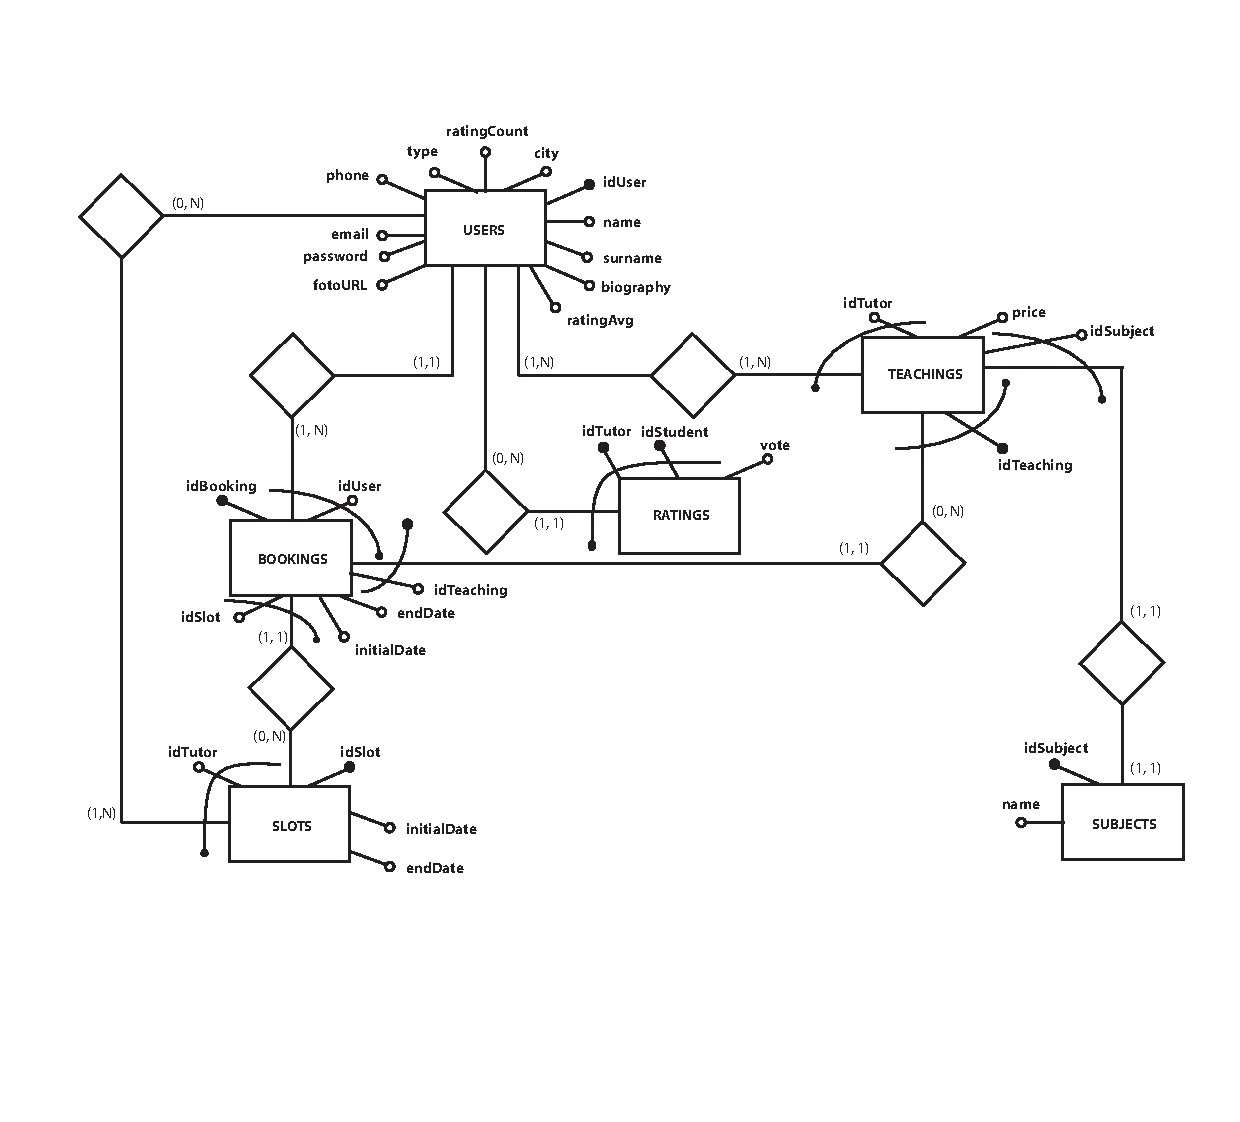
\includegraphics[width=\textwidth]{../../interni_statici/ER.pdf}
	\caption{Diagramma ER}
	\label{fig:er}
\end{figure}


\pagebreak
\section{Accessibilità}
Per cercare di rendere la piattaforma il pi\`u usabile possibile e venire incontro alle esigenze del maggior numero di utenti si \`e deciso di adottare una serie di accorgimenti atti ad incrementare l'accessibilit\`a del sito. Molti di questi sono stati utilizzati seguendo lo standard WCAG 2.0 (Web Content Accessibility).

\subsection{Palette di colori}
Tutti i colori utilizzati per la realizzazione delle pagine sono stati scelti sia perseguendo un'estetica accattivante che tenendo conto del livello di accessibilità che essi permettono. In particolare, si \`e data importanza al livello di contrasto tra i colori utilizzati nel sito; il rapporto target \`e stato fissato ad un livello di contrasto \emph{AAA}, che per il \emph{WCAG 2.0} corrisponde ad un fattore pari ad almeno \emph{7:1}.\\
\`E stato inoltre utilizzato il tool per il calcolo del rapporto di contrasto messo a disposizione all'indirizzo \url{http://www.http://leaverou.github.io/contrast-ratio/}\\\\
Il \textbf{template} applicato alle pagine del sito comprende principalmente i seguenti colori:

\begin{multicols}{2}
	\begin{center}
		\begin{tabular}{|c|c|c|}
			\hline
			\textbf{Posizione} & \textbf{codice}\\
			\hline
			Header & \#23282D \\
			\hline
			Header-Links & \#F9FBFD \\
			\hline
			Body-Background & \#2B3137 \\
			\hline
			Body-Text & \#D5D5D5 \\
			\hline
			Body-Links & \#7ABBDC \\
			\hline
		\end{tabular}
	\end{center}
	
	\begin{center}
		\begin{tabular}{|c|c|c|}
			\hline
			\textbf{Codice A} & \textbf{Codice B} & \textbf{Rapporto}\\
			\hline
			\#2B3137 & \#D5D5D5 & 8.96\\
			\hline
			\#23282D & \#F9FBFD & 14.3\\
			\hline
			\#2B3137 & \#7ABBDC & 7.1\\
			\hline
		\end{tabular}
\end{center}
\end{multicols}
Dove nella tabella di sinistra vengono i riportati i codici colore assegnati ad un particola sezione della pagine, mentre nella colonna di sinistra sono riportati i rapporti di contrasto tra i codici colore \emph{A} e \emph{B}.\\\\

Per quanto riguarda invece le \textbf{caselle di input}, sono stati utilizzati i colori riportati in tabella (a sinistra), i cui rapporti sono riportati nella tabella di destra:
\begin{multicols}{2}
\begin{center}
		\begin{tabular}{|c|c|c|}
			\hline
			\textbf{Posizione} & \textbf{codice}\\
			\hline
			Background & \#2B3137 \\
			\hline
			Labels & \#D5D5D5 \\
			\hline
			Text & \#7ABBDC \\
			\hline
		\end{tabular}
	\end{center}
	
\begin{center}
		\begin{tabular}{|c|c|c|}
			\hline
			\textbf{Codice A} & \textbf{Codice B} & \textbf{Rapporto}\\
			\hline
			\#2B3137 & \#D5D5D5 & 14.3\\
			\hline
			\#2B3137 & \#7ABBDC & 12.7 \\
			\hline
		\end{tabular}
\end{center}
\end{multicols}
\pagebreak
\subsection{Codice HTML}
Vengono riportati di seguito una serie di accorgimenti apportati al codice \emph{HTML} delle pagine per rendere il sito pi\`u accessibile.
\begin{itemize}
	\item \textbf{title tag}: per agevolare il \emph{bookmarking} si sono resi i titoli
	\begin{itemize}
		\item brevi e concisi;
		\item descrizione dal particolare al generale.
	\end{itemize}
\end{itemize}
\begin{itemize}
	\item \textbf{h tag}: tutti i \emph{tag h} sono semanticamente coerenti con il contenuto delle pagine;
	\begin{itemize}
		\item brevi e concisi;
		\item descrizione dal particolare al generale.
	\end{itemize}
\end{itemize}
\begin{itemize}
	\item \textbf{img tag}:
	\begin{itemize}
		\item gli attributi \emph{alt} sono presenti e non vuoti.
	\end{itemize}
\end{itemize}
\begin{itemize}
	\item \textbf{a tag}: particolare attenzione \`e stata rivolta ai link
	\begin{itemize}
		\item avviene sempre un cambiamento nella colorazione dei link \emph{visited};
		\item il link della pagina corrente viene visualizzato sottolineato;
		\item sono stati inserti gli attributi title per dare una maggiore coerenza;
		\item si \`e tolta la possibilit\`a di cliccare il link della pagina in cui ci si trova.
	\end{itemize}
\end{itemize}

\end{document}
